\documentclass[11pt,a4paper]{article}

% Packages
\usepackage[utf8]{inputenc} % Encoding
\usepackage[T1]{fontenc}   % Font encoding
\usepackage{amsmath,amssymb,amsfonts} % Math packages
\usepackage{graphicx}      % For including graphics
\usepackage{xcolor}        % For colored text
\usepackage{hyperref}      % For hyperlinks
\usepackage{geometry}      % For page layout
\usepackage{float}         % For better float placement
\usepackage{enumitem}      % For custom lists
\usepackage{caption}       % For captions
\usepackage{subcaption}    % For subfigures
\usepackage{listings}
\usepackage{csvsimple}  % Package for handling CSV files

\lstset{
  basicstyle=\ttfamily\small,  % Use small monospaced font
  keywordstyle=\color{blue},  % Set color for keywords
  commentstyle=\color{green},  % Set color for comments
  stringstyle=\color{red},  % Set color for strings
  breaklines=true,  % Enable line breaking for long lines
  frame=single,  % Add a frame around the code
  showstringspaces=false  % Don't show spaces in strings
}
% Geometry settings
\geometry{
  a4paper,
  left=1in,
  right=1in,
  top=1in,
  bottom=1in
}

% Custom commands

% Title and Author
\title{CSE-368 Final Project Report}
\author{Jacob DeRosa, Saqib Malik}
\date{\today}

\begin{document}

% Title Page
\maketitle
\tableofcontents
\newpage

% Sections
\section{Introduction}
AssaultCube is a 3D first-person shooter from 2006. It's based on the Cube engine written in C++. Assault Cube features a variety of game modes that include team based combat, we will focus on the free for all deathmatch gamemode. The goal of each player is to accumulate the most number of eliminations. Artificial intelligence (AI) plays a big role in enhancing gameplay. Specifically, in games like AssaultCube, AI algorithms are used in enemy/ally bots for enabling numerous capabilities such as pathfinding to areas of interest and targeting enemies. These features of the built-in AssaultCube bots add to the immersive and unpredictable nature of the game. In this project, we implemented a different flavor of AI bot that accomplishes many of the objectives of the built-in bots. To implement this, we developed custom \textbf{detour hooking} code to patch the main gameplay loop, adding an adaptive decision-making algorithm that will control our AIs movement, pathfinding, and targeting decisions. Our agent is able to continuously learn, remember routes and solve problems unlike the Assault-Cube agents giving it an advantage over enemies.

\section{Technologies \& Techniques Explored}
The initial technologies investigated were machine-learning based. We decided on trying our hand at implementing a reinforcment-learning agent using existing libraries. Two notable libraries explored were Tensorflow and mlpack. Conditional techniques and graph based decision making were later considered as a more straightforward approach later in the project due to time constraints and overall complexity vs. performance.

Both \textbf{Tensorflow} and \textbf{mlpack} are machine-learning libraries for Python and C++, respectively. Tensorflow had high consideration due to its robust framework and well-established libraries, it was also in a more familiar Python environment. It was ultimately determined to not be as suitable for the project requirements because it would’ve required a complex memory-sharing setup between different processes to accomplish properly as well as creating python bindings between the AI and the hook code. While mlpack would be straightforward and could run under the same process as the game as it is C++, it posed the challenge of potentially long training times and lack of training resources. Like bots that are already implemented in AssaultCube, an adaptive conditional-based algorithm was chosen for the AI. These Bots utilize a pre-made graph for each path and the A-Star pathfinding algorithm. Being able to control the condition-actions, level of learning, and overall algorithm gave more flexibility in how the AI is controlled. This algorithm was injected into AssaultCube via GDB, which would run the agent process once per game-tick.

Our group was familiar with Tensorflow due to its popularity as a Python machine-learning library, although not every member had hands-on experience with it. The discovery of mlpack came from researching machine-learning libraries specific to a C++ environment. A conditional-based algorithm idea came from work done in class. Specifically, homework assignments like Pacman AI, where we would assign reward values to certain game states to determine what comes next. Conditional AIs are also very common for games to use in general, they provide a way for developers to make simple rules for bots to follow without complicating their mechanics.

I am also testing the same algorithm refactored in omp so that I can run it on a CCR0-CPU node to compare the performance. I chose the n domain to start at 2 thousand and proceed by powers of 2 untill $256e3$. I am starting at 1 core to get T\_1 and proceeding by powers of 2 until 64 cores.

\section{Methods \& Methodology}
To begin, we needed to programmatically set up an environment that our agent could interact with. This process involved a fair amount of game reverse engineering, and low-level knowledge of instruction processing. We successfully developed a custom detour hooking method that was applied to a function called \textit{checkinput()} in the game’s main loop. This allowed us to have our own code that ran once per frame. Once we had runnable code inside the game we could extract relevant information related to the player and the current environment. The game could also be controlled simulating an actual human controlling the game via our injected code. 

Once we could run our own code in the game, we moved on to implementing various pieces of artificial intelligence into our custom bot. Our chosen environment consisted of a custom-made map, Ground Zero, along with the built-in AssaultCube bot deathmatch maps. Since we had access to all details of the player, and other players, we could pull that info any time we needed. Two general algorithms were developed in sequence: aimbot and navigating/targeting.

\subsection{Aimbot}
The aimbot algorithm was relatively simply and consistent. At a high-level, when an enemy is seen, aim at them and shoot until eliminated. This algorithm is best described with the following sequence: 
	\begin{enumerate}
    \item Loop over dynamic entities (other players) until a non-dead player is found. 

    \item Check if player is on-screen (in front of you whether obstructed or not).

    \item Check if player is visible (not obstructed by another player or wall/object). 

    \item Aim at the player. 

    \item Fire until player is eliminated. 
	\end{enumerate}

One of the purposes of our AI is to be realistic, so not necessarily cheat. The AI would only aim at an enemy if it could see them, similar to a real human, rather than target-locking all enemies and running towards them. To achieve this, we had to make sure that an enemy player is on-screen, and also not obstructed by any object (or another player). Determining if a player is on-screen is simply a result of matrix multiplication involving the Model-View-Projection matrix and player XYZ coordinates. If the resulting output is a valid screen coordinate (within the bounds of the game resolution and non-negative), then the player is on-screen. 

\begin{figure}[H]
    \centering
    \begin{minipage}[b]{0.45\textwidth}
        \centering
        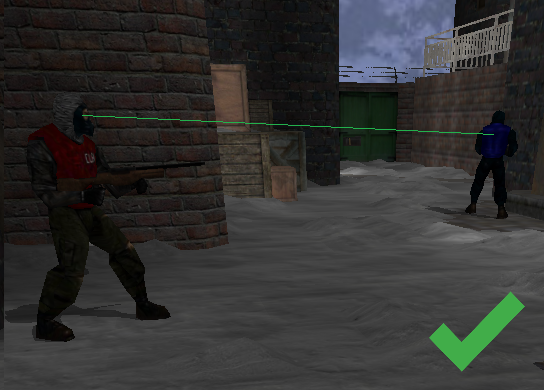
\includegraphics[width=\textwidth]{tracelineCollision.png}
        \caption{AI Detecting Another Player}
        \label{fig:one}
    \end{minipage}
    \hfill
    \begin{minipage}[b]{0.45\textwidth}
        \centering
        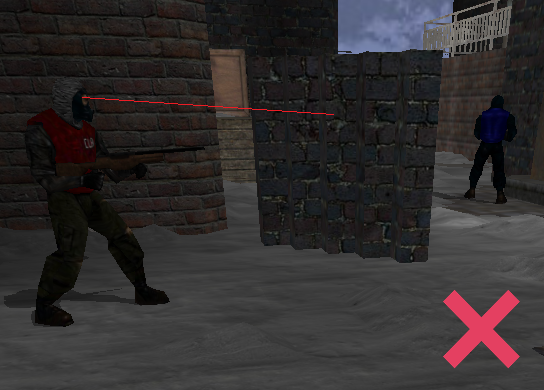
\includegraphics[width=\textwidth]{tracelineNoCollision.png}
        \caption{AI Vision Blocked (No Detection)}
        \label{fig:two}
    \end{minipage}
\end{figure}

\subsection{Navigation \& Targeting}
The development of the modern navigation algorithm took about a month in total and is slightly different from the first used approach. The navigation for the agent is graph based and follows several design characteristics. It needs to be able to learn, unlearn and remember paths. Paths in the graph represent a series of points on the map that the agent can follow progressively without getting stuck. It also needs to be able to overcome obstacles, such as tiny rooms, boxes, ledges, fences. It needs to be approximate paths to targets outside the graph reliably. This long list of requirements seems very complicated and daunting but we were able to develop a relatively simple algorithm that posseses all of these characteristics while remaining computationally efficient.

The core of the algorithm is divided into 2 parts, vision and pathfinding. To see the map we reversed the TraceLine function from the game to draw rays from our target until it collides with the map. Pathfinding is simply BFS because we aren't looking for optimal paths we are just approximating the map. BFS is a simple, reliable, and efficient algorithm which allows us to use it extensively in the agents decision making process. These are all the tools we needed to implement the navigation algorithm that follows.

This algorithm starts by initializing an empty graph framework where we have a predetermined number of spaces where nodes can be allocated, currently the agent is running on 2048 nodes. The node id's are associated with the index of two lists, \textit{connected\_pool} and \textit{free\_pool}. Edges are stored in an adjacency matrix and node positions are stored in another list. Its important to note that when we drop the agent into the game it basically knows nothing about its environment. Graph nodes may be allocated and deallocated and edges can be cut or added at any point during the game. The most important piece is the objectives stack which holds the current path for the agent consisting of node ids.

First we update our objective velocity which is how we measure the rate of change to the next node. Then we update the target position, this takes the closest enemy and logs their position. 
When the player reaches an a node we pop it off the stack and set it to the current node, then we discover routes. This involves taking the closest $k$ nodes and drawing rays to them. All the non-colliding rays are added as new edges to the graph. Next we see if the objectives is empty meaning we have finished a BFS path. If it is we perform a \textbf{Scan}, this means the agents picks $k$ random yaw points and draws a ray until it collides with the map, we calculate where $2/3$ of the distance along the ray is on the map and add it as a new node to the graph. Anytime a Scan is performed we call the self optimizing capability of the algorithm called \textbf{Prune}. Prune is called when there are no more free nodes to allocated. It ends up removing $\sqrt{nodes}$ from the graph using the heuristic $cardinality(x)*sumSquaredDistances(x)$ for each node and sorting in ascending order. This removes nodes that are close to lots of other nodes and have few edges which will overtime allow the graph to balance itself and learn larger routes.

Next we evaluate if we are in proximity of a jump node and jump if we are. Then we check if the objective velocity is very close to 0 (we are stuck). If we are stuck and there is no existing jump node  request we can enable one. A jump node request places an intermediary node on the path and evaluates the accumulated objective distance covered to see if its a valid spot to jump. If it is we add it to the graph and reconfigure the edges. Otherwise we remove the current objective and perform a Scan to unstick the agent.

Then the agent checks if the objectives are set and if not it finds the closest node to the target and BFS's to that node. If the graph was cut into multiple partitions and that node isn't reachable the agent proceeds to find the closest connected node it can actually access. The BFS path is stacked onto the objectives. If the agent finds itself outside the graph for some reason, BFS was not successful we simply Prune and Scan until it finds the graph again.

This is a continuously learning approximation algorithm that can self optimize and play on any map without needing to hardcode objectives. Its very robust and almost all atempts to make it stuck were unsuccessfult except for throwing it down a well. Graph pruning is implemented in a way that means more edges cover more area of the map and allow the agent to learn massive complex spaces with relatively little complexity. It also has some hyperparameters we can tweak to change the learning behavior and capabilities like k and the max number of nodes.

\section{Performance Evaluation}

Our AI is capable of exploration, targeted pathfinding, and eliminating opponents. In runs of the AI we observe it doing the following things:

	\begin{enumerate}
    \item Slowly exploring the area around it.

    \item Targeting enemies when they are seen.

    \item Prioritizing high-kill areas (areas where enemies are more likely to be seen).
	\end{enumerate}

The metric used to determine the success of the AI is the exploration and kill-rate of AI movement versus randomized movement. Randomized movement, for the sake of this project, is defined as moving forward, backward, left, right, or diagonal along with randomly looking around at an angle perpendicular to the floor. Randomized movement follows no matching behavior to AI movement, other than the aimbot system (in order to observe kill-rates fairly). Exploration is defined as the number of unique X, Y coordinates visited under each algorithm. For example, visiting coordinates (1, 1), (2, 1) then (1, 1) would constitute two unique explorations. Kill-rate is simply number of eliminations the algorithm has achieved. The following results were achieved by running the algorithms on Bot Deathmatch, versus three bots (bad difficulty), on the map \textit{ac\_africa}.

\begin{figure}[H]
    \centering
    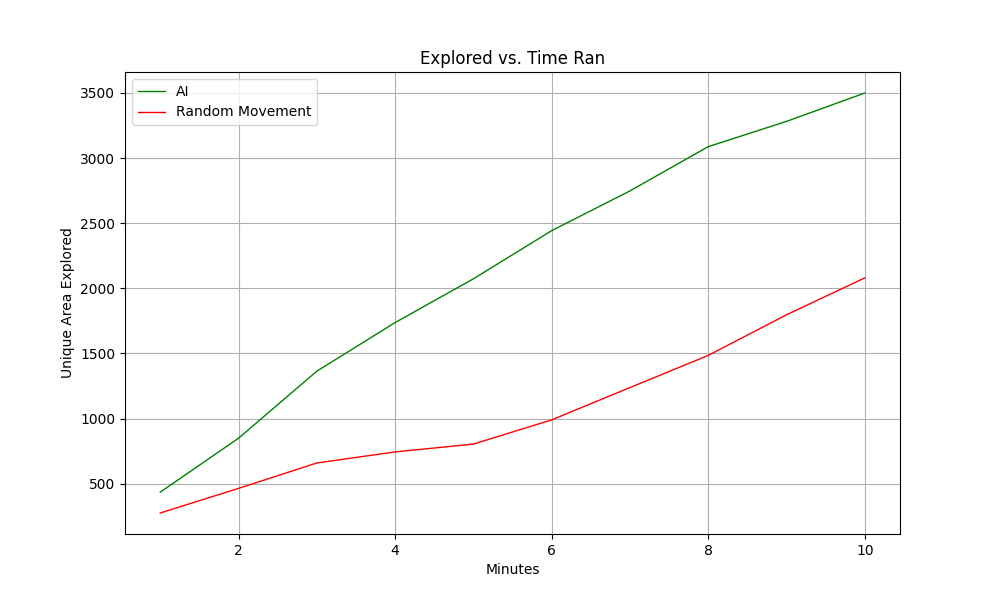
\includegraphics[width=0.8\textwidth]{areaExploredGraph.png}
    \caption{AI versus randomized algorithm movement.}
    \label{fig:three}
\end{figure}
\begin{figure}[H]
    \centering
    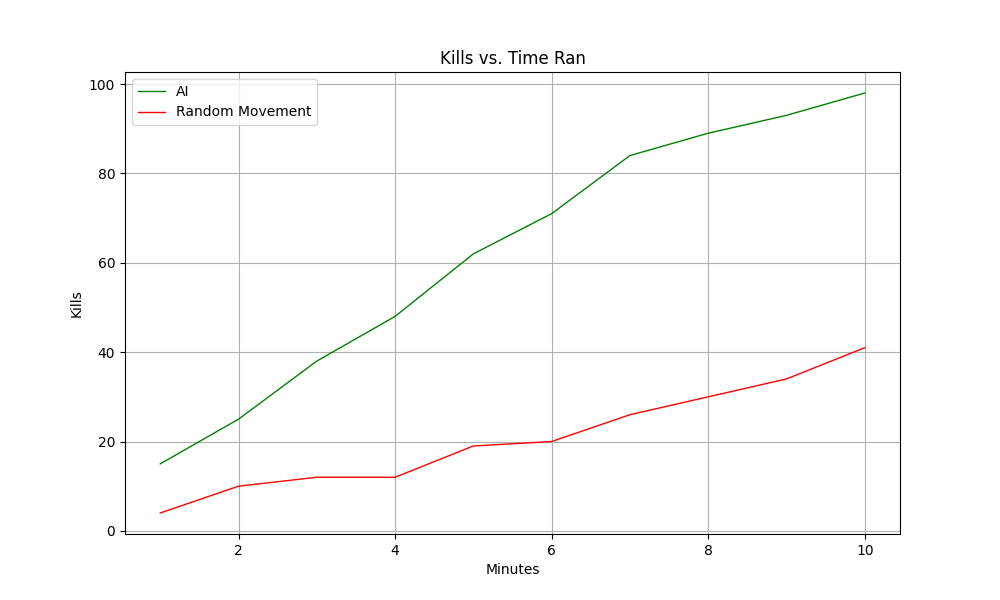
\includegraphics[width=0.8\textwidth]{killsGraph.png}
    \caption{AI versus randomized algorithm kill-rate.}
    \label{fig:four}
\end{figure}

The results overwhelming indicate the success of the AI as opposed to random movement. This success is a result of the AI behaving cleverly in comparison to the random movement. The hyperfocus on eliminating enemies and sticking to areas that have higher enemy concentration clearly assists it in achieving its goals.

\section{Conclusion}
The biggest skills picked up during this project was our unique way of interacting with the environment. Rather than rely on the open-source code and compile our AI directly into the game, we inject the AI’s code into the running process of the game. Similarly to the HW projects, we gained more experience with weighing certain decisions over another. Decisions like whether to be exploring, pathfinding to an enemy, attempting to jump over obstacles, or shooting at an enemy. While on paper not sounding too difficult, implementing in a 3D environment posed a challenge when compared to the 2D environment of games like Pacman. We had to account for the yaw and pitch of the AI and its XYZ. 

We are satisfied with how our AI has developed. Going back, if we could have handled code injection and environment setup sooner/cleaner more work could have been done for the AI. Having experimented with machine-learning algorithms would have been a very good learning experience, although we figured we may not have enough time to train a model properly. We think that a machine-learning approach is the next best step for this sort of AI. Conditional-based AI is commonly used in videogames, whereas any sort of adaptive ML-based AI is rarer. The potential for a more robust AI that learns from analyzing other players or its own gameplay will be one of the next revolutionary steps in the gaming industry. 

\enlargethispage{14\baselineskip}
\section{Resources}
\begin{table}[H]
    \begin{tabular}{|p{0.3\textwidth}|p{0.6\textwidth}|}
        \hline
        \textbf{Source} & \textbf{Description} \\ \hline
        \href{https://github.com/VX59/cse-368-team-project}{Project Repo (Link)} & Repo hosting code for this paper. \\ \hline
        \href{https://github.com/assaultcube/AC}{AssaultCube Source (Link)} & Source code of AssaultCube. \\ \hline
        \href{https://github.com/faluthe/vtable-hook}{V-Table Guide (Link)} & Reference for v-table hooking (by Falu). \\ \hline
        \href{https://github.com/microsoft/Detours/wiki}{Detours Wiki (Link)} & Detour hooking resources. \\ \hline
        Lecture 2 & Uninformed Search \& Graphs (BFS) \\ \hline
    \end{tabular}
\end{table}
\end{document}